\documentclass[11pt,a4paper]{article}
\usepackage{fontspec}
\defaultfontfeatures{Ligatures=TeX}
\setmainfont{Latin Modern Roman}
\setsansfont{Latin Modern Sans}
\setmonofont{Latin Modern Mono}
\IfFontExistsTF{Noto Serif CJK SC}{\newfontfamily\zhfont{Noto Serif CJK SC}}{\newfontfamily\zhfont{FandolSong-Regular}}
\usepackage[margin=1in,headheight=15pt,headsep=14pt]{geometry}
\usepackage{amsmath,amssymb,bm,graphicx,booktabs,tabularx,array,longtable}
\usepackage{tikz,caption,enumitem,fancyhdr,microtype,xurl,listings}
\usetikzlibrary{positioning,arrows.meta}
\usepackage[section]{placeins}
\usepackage[hidelinks,unicode]{hyperref}
\usepackage[nameinlink,noabbrev]{cleveref}
\newcommand{\TeamNumber}{856}

\definecolor{sourceRed}{RGB}{176,58,46}
\definecolor{sourceOrange}{RGB}{224,138,60}
\definecolor{sourceGreen}{RGB}{46,125,50}
\definecolor{sourceBlue}{RGB}{31,78,121}
\definecolor{sourcePurple}{RGB}{106,61,154}
% Source PNG bytes remain unchanged. Only label regions are typeset over in LaTeX.
\newcommand{\SourceHistory}[3]{%
\begin{tikzpicture}
\node[anchor=south west,inner sep=0] (im) at (0,0) {\includegraphics[width=\linewidth]{#1}};
\begin{scope}[x={(im.south east)},y={(im.north west)}]
\fill[white] (0,.14) rectangle (.042,.91);
\fill[white] (0,0) rectangle (1,.085);
\fill[white] (0,.915) rectangle (1,1);
\node[rotate=90,font=\small] at (.021,.52) {#2};
\node[font=\small] at (.53,.045) {Time after separation $t$ (s)};
\node[font=\small] at (.53,.97) {#3};
\end{scope}
\end{tikzpicture}}
\newcommand{\SourceTrajectory}{%
\begin{tikzpicture}
\node[anchor=south west,inner sep=0] (im) at (0,0) {\includegraphics[width=\linewidth]{source9.png}};
\begin{scope}[x={(im.south east)},y={(im.north west)}]
\fill[white] (0,0) rectangle (1,.085);
\fill[white] (0,.925) rectangle (1,1);
\fill[white] (0,.13) rectangle (.037,.91);
\fill[white] (.565,.13) rectangle (.593,.91);
\node[rotate=90,font=\footnotesize] at (.019,.52) {Altitude $h$ (km)};
\node[rotate=90,font=\footnotesize] at (.581,.52) {Altitude $h$ (km)};
\node[font=\footnotesize] at (.295,.045) {Surface range $s$ (km)};
\node[font=\footnotesize] at (.795,.045) {Surface range $s$ (km)};
\node[font=\footnotesize] at (.295,.968) {(a) Full trajectory; dots: landing ignition};
\node[font=\footnotesize] at (.795,.968) {(b) Terminal region below 60 km};
\fill[white] (.437,.68) rectangle (.542,.916);
\foreach \yy/\cc/\txt in {.885/sourceRed/{90 t (fail)},.840/sourceOrange/{110 t},.795/sourceGreen/{130 t},.750/sourceBlue/{150 t},.705/sourcePurple/{200 t}}{
\draw[\cc,line width=1pt] (.442,\yy)--(.464,\yy);
\node[anchor=west,font=\scriptsize] at (.470,\yy) {\txt};}
\end{scope}
\end{tikzpicture}}
\newcommand{\SourceFuelPlot}{%
\begin{tikzpicture}
\node[anchor=south west,inner sep=0] (im) at (0,0) {\includegraphics[width=\linewidth]{source13.png}};
\begin{scope}[x={(im.south east)},y={(im.north west)}]
\fill[white] (0,0) rectangle (1,.085);
\fill[white] (0,.915) rectangle (1,1);
\fill[white] (0,.16) rectangle (.042,.91);
\node[rotate=90,font=\small] at (.021,.53) {Propellant consumed (t)};
\node[font=\small] at (.53,.045) {Initial total propellant $m_{p,0}$ (t)};
\node[font=\small] at (.53,.969) {Propellant allocation across the baseline load scan};
\fill[white] (.106,.74) rectangle (.252,.905);
\draw[dashed,line width=.8pt] (.113,.87)--(.14,.87);
\node[anchor=west,font=\scriptsize] at (.15,.87) {Available load};
\fill[sourceBlue] (.113,.81) rectangle (.14,.835);
\node[anchor=west,font=\scriptsize] at (.15,.823) {Entry burn};
\fill[sourceRed] (.113,.76) rectangle (.14,.785);
\node[anchor=west,font=\scriptsize] at (.15,.773) {Landing burn};
\fill[white] (.276,.82) rectangle (.39,.905);
\node[anchor=west,font=\scriptsize,text=sourceGreen] at (.28,.875) {$\sim105$ t};
\node[anchor=west,font=\scriptsize,text=sourceGreen] at (.28,.838) {graphical estimate};
\end{scope}
\end{tikzpicture}}
\newcommand{\SourceAttitudePlot}{%
\begin{tikzpicture}
\node[anchor=south west,inner sep=0] (im) at (0,0) {\includegraphics[width=\linewidth]{source14.png}};
\begin{scope}[x={(im.south east)},y={(im.north west)}]
\fill[white] (0,0) rectangle (1,.088);
\fill[white] (0,.915) rectangle (1,1);
\foreach \xx in {.171,.523,.865}{\node[font=\scriptsize] at (\xx,.04) {Time $t$ (s)};}
\node[font=\scriptsize] at (.175,.969) {(a) RCS reorientation};
\node[font=\scriptsize] at (.523,.969) {(b) Required thrust direction};
\node[font=\scriptsize] at (.865,.969) {(c) Moment scales};
\foreach \xa/\xb in {0/.028,.325/.348,.350/.372,.668/.688,.690/.711}{\fill[white] (\xa,.14) rectangle (\xb,.90);}
\node[font=\tiny,rotate=90,text=sourceBlue] at (.015,.52) {Rotation angle (deg)};
\node[font=\tiny,rotate=90,text=sourceRed] at (.337,.52) {Angular rate (deg/s)};
\node[font=\tiny,rotate=90] at (.361,.52) {Thrust angle (deg)};
\node[font=\tiny,rotate=90,text=sourceRed] at (.678,.52) {Direction rate (deg/s)};
\node[font=\tiny,rotate=90] at (.701,.52) {Moment (N m)};
\fill[white] (.873,.10) rectangle (.989,.32);
\draw[sourceGreen,line width=.8pt] (.88,.27)--(.90,.27);\node[anchor=west,font=\tiny,inner sep=0pt] at (.900,.27) {Aerodynamic};
\draw[sourceRed,dashed,line width=.8pt] (.88,.21)--(.90,.21);\node[anchor=west,font=\tiny,inner sep=0pt] at (.900,.21) {TVC, $5^\circ$};
\draw[sourceBlue,dotted,line width=.8pt] (.88,.15)--(.90,.15);\node[anchor=west,font=\tiny,inner sep=0pt] at (.900,.15) {Grid fins};
\end{scope}
\end{tikzpicture}}

\graphicspath{{../../results/figures/}{figures/}}
\captionsetup{font=normalsize,labelsep=period,labelfont=normalfont}
\captionsetup[table]{position=top}
\setlength{\parindent}{17pt}
\setlength{\parskip}{0pt}
\setlength{\emergencystretch}{2em}
\setlist{itemsep=2pt,topsep=4pt,parsep=0pt}
\setcounter{tocdepth}{2}
\makeatletter
\renewcommand*\l@subsection{\@dottedtocline{2}{1.5em}{2.6em}}
\setlength{\@fptop}{0pt}
\setlength{\@fpsep}{18pt}
\makeatother
\pagestyle{fancy}
\fancyhf{}
\fancyhead[L]{Problem A}
\fancyhead[R]{Team \TeamNumber}
\fancyfoot[C]{\thepage}
\renewcommand{\headrulewidth}{.4pt}
\newcommand{\vect}[1]{\bm{#1}}
\hypersetup{pdftitle={Simulation of a Seven-Engine Recoverable Booster with Two-Phase Retropropulsion},pdfauthor={Team \TeamNumber}}
\begin{document}
\hypersetup{pageanchor=false}
\thispagestyle{fancy}
\pagenumbering{gobble}
\begin{center}
\vspace*{6mm}
{\LARGE\bfseries Simulation of a Seven-Engine Recoverable Booster\par with Two-Phase Retropropulsion\par}
\vspace{5mm}
{\large Team \TeamNumber, Problem A\par}
\vspace{6mm}
{\large\bfseries Abstract\par}
\end{center}
\noindent
This paper presents the simulation study of a 130 t dry-mass booster separating at 70 km altitude with a speed of 6,000 km/h and an upward flight-path angle of $45^\circ$. Seven methane--oxygen engines support entry braking and terminal descent. The study combines variable mass, altitude-dependent gravity, atmospheric density, Mach-dependent drag, wind, and state-dependent guidance, and examines initial propellant loads between 90 and 200 t.

The final combined model supports a recommended separation propellant load of 110--112 t. At 110 t, it consumes 106.6 t, retains 3.4 t, and reaches a touchdown speed of 2.02 m/s. This final result includes attitude-dependent area, finite engine response, and staged engine selection. Earlier baseline, parameterized, and combined-model scans give lowest tested passing loads of 104, 96, and 102 t, respectively; these are development-stage thresholds rather than alternative final recommendations. Baseline entry consumption is about 40--44 t, and terminal consumption grows with carried mass. A version register separates the calculation series and the diagnostic comparisons.

Separate crosswind, reaction-control, and jet-interaction analyses characterize effects omitted from the simplest baseline. The findings emphasize the interaction between burn timing, carried mass, throttle floor, and engine-count staging. These results belong to distinct model versions; their empirical thresholds are not global minimum-fuel proofs. Heating, fully coupled attitude/contact dynamics, and the completeness of uncertainty coverage remain limitations.
\clearpage
\hypersetup{pageanchor=true}
\pagenumbering{roman}
{\small\tableofcontents}
\clearpage
\pagenumbering{arabic}

\section{Introduction}
\subsection{Problem background and restatement}
Recovering a first-stage booster requires a controlled return from high speed to a nearly vertical, low-speed arrival at a ship. Atmospheric drag assists the descent, but the same flow produces pressure loads and wind-induced deviations. Propellant retained at separation increases braking capability while also increasing the mass that must be decelerated. Burn timing and engine selection therefore influence both fuel consumption and terminal control.

The booster has dry mass 130,000 kg, height 65 m, diameter 7.0 m, and seven 1 MN-class liquid-oxygen/methane engines. Separation occurs at 70 km with speed 1,666.667 m/s and flight-path angle $+45^\circ$. The ship can be positioned downrange as allowed by the competition problem \cite{problem}. Initial total propellant is varied from 90 to 200 t, followed by finer scans near the feasibility boundaries of the refined models.


\begin{figure}[htbp]
\centering
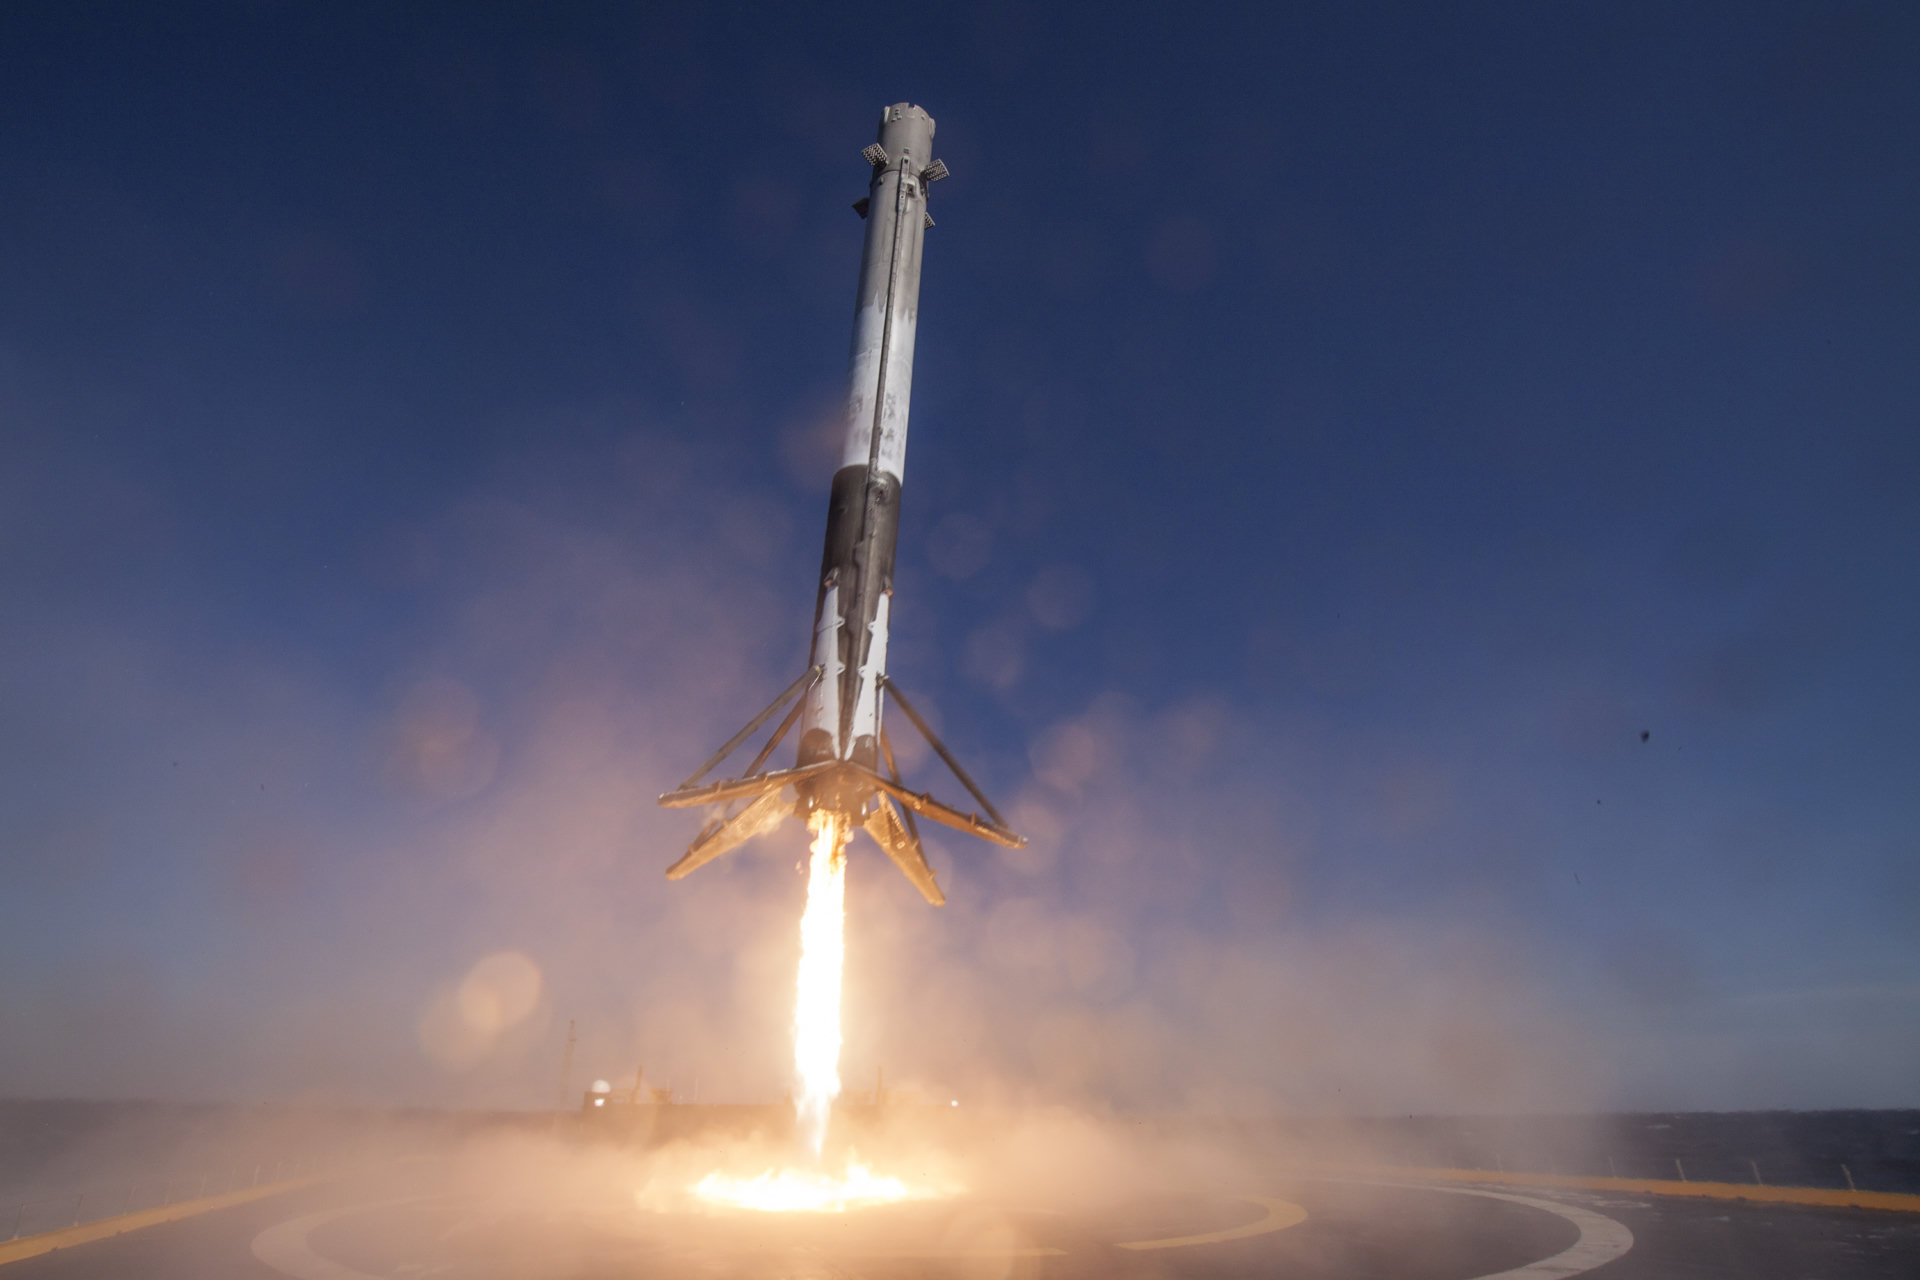
\includegraphics[width=.82\linewidth,height=.30\textheight,keepaspectratio]{figures/booster_photo.jpg}
\caption{A Falcon 9 booster during a powered droneship landing (CRS-8). Photograph: SpaceX, CC0. The photograph illustrates the recovery context; the modeled seven-engine vehicle is hypothetical.}
\label{fig:recovery_photo}
\end{figure}

\subsection{Objectives and study organization}
The study addresses four questions: how the ascent and return arc develop after upward separation; how entry and terminal burns divide the propellant budget; whether reduced loads remain feasible under the reported perturbations; and how area coupling, engine transients, and engine-count changes modify the load recommendation.

The analysis distinguishes baseline guidance, parameterized guidance, and actuator refinements. Their thresholds and recommendations are compared within their respective assumptions and perturbation sets.

\begin{figure}[htbp]
\centering
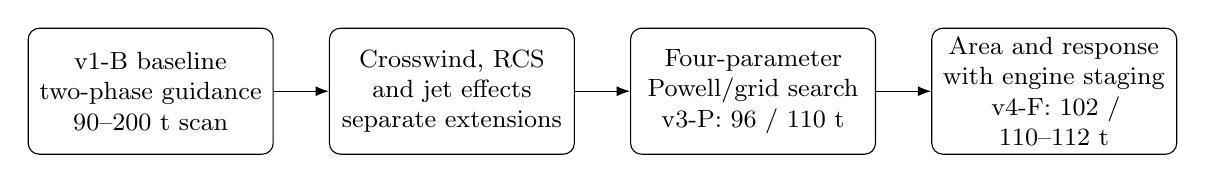
\begin{tikzpicture}[>=Latex,node distance=7mm,
box/.style={draw,rounded corners,align=center,font=\small,text width=29mm,minimum height=16mm,inner sep=3pt}]
\node[box] (a) {v1-B baseline\\ two-phase guidance\\90--200 t scan};
\node[box,right=of a] (b) {Crosswind, RCS\\and jet effects\\separate extensions};
\node[box,right=of b] (c) {Four-parameter\\Powell/grid search\\v3-P: 96 / 110 t};
\node[box,right=of c] (d) {Area and response\\with engine staging\\v4-F: 102 / 110--112 t};
\draw[->] (a)--(b);\draw[->] (b)--(c);\draw[->] (c)--(d);
\end{tikzpicture}
\caption{Organization of the simulation study. The successive boxes describe reported study stages, not a claim that every physical extension was coupled into one validated simulator. Nominal thresholds and recommended loads belong to their respective versions.}
\label{fig:workflow}
\end{figure}

\section{Assumptions, Parameters, and Notation}
\subsection{Reference assumptions}
The baseline motion is described in the vertical plane determined by the separation velocity and Earth center. Gravity varies with altitude, mass decreases as propellant is expelled, and drag is evaluated relative to the prescribed wind. The baseline guidance treats attitude alignment as ideal; later sections introduce separate attitude estimates and a first-order lag.

The initial trajectory is upward, with an apogee near 143 km. The atmospheric representation therefore includes an exponential continuation above 86 km, together with a Mach-dependent drag coefficient.

\begin{table}[htbp]
\caption{Parameters of the simulation study.}
\label{tab:src4}
\small
\setlength{\tabcolsep}{3.5pt}
\begin{tabularx}{\linewidth}{@{}p{.26\linewidth}p{.36\linewidth}X@{}}
\toprule
Parameter & Value & Basis / status \\
\midrule
Dry mass; dimensions & 130 t; 65 m; 7.0 m & Problem data (G) \\
Separation altitude; speed & 70 km; 1666.667 m/s & Problem data (G) \\
Initial flight-path angle & $45^\circ$ & Scenario (H) \\
Engine system & $7\times1$ MN; $I_{sp}=330$ s & Virtual reference (H) \\
Oxygen/methane ratio & 3.4 & Scenario (H) \\
Reference area & 38.4845 m$^2$ & Derived from diameter (D) \\
Mach-dependent drag & 12 anchors; maximum $C_D=1.50$ & Simulation drag model (H) \\
Atmosphere & USSA 1976 layers; exponential above 86 km & Reference plus extension \\
Earth & $R_E=6371$ km; $\mu=3.986\times10^{14}$ m$^3$/s$^2$ & Reference constants \\
Wind profile & Height-dependent; see Table~\ref{tab:src3} & Scenario (H) \\
Pressure limit & 50 kPa & Screening target (H) \\
Target touchdown speed & 1.5 m/s; baseline test below 3 m/s & Guidance and acceptance choices (H) \\
\bottomrule
\end{tabularx}
\par\smallskip{\footnotesize Shared problem data and reference assumptions; calculation-series identifiers are listed in \cref{tab:versions}. See \cref{tab:versions}.}
\end{table}


G denotes problem data, H a scenario or modeling assumption, and D a value derived from the geometry. The drag representation has 12 anchors and a peak coefficient of 1.50. The complete anchor set and the high-altitude scale height require specification for independent numerical reproduction.

\subsection{Notation and angular convention}
\begingroup
\small
\begin{longtable}{@{}p{0.17\linewidth}p{0.77\linewidth}@{}}
\caption{Notation used to express the study model.}\label{tab:notation}\\
\toprule Symbol & Meaning\\ \midrule
\endfirsthead
\toprule Symbol & Meaning (continued)\\ \midrule
\endhead
\bottomrule\endfoot
$s$ & Surface range\\
$h$ & Altitude\\
$r$ & Geocentric radius\\
$R_E$ & Earth radius\\
$u$ & Horizontal ground velocity\\
$w$ & Vertical ground velocity\\
$V_g$ & Ground speed\\
$V_{rel}$ & Air-relative speed\\
$m$ & Total vehicle mass\\
$m_{p,0}$ & Initial total propellant mass\\
$T$ & Thrust magnitude\\
$D$ & Drag magnitude\\
$\beta_h$ & Thrust angle from the local horizontal in the force equations\\
$\chi$ & Drag-direction angle\\
$\gamma$ & Flight-path angle\\
$\theta_T$ & Reported thrust deflection from the upward vertical\\
$\rho$ & Air density\\
$C_D$ & Drag coefficient\\
$M$ & Mach number\\
$q$ & Dynamic pressure\\
$h_e$ & Entry ignition height\\
$v_{cut}$ & Entry cutoff speed\\
$k$ & Terminal ignition multiplier\\
$V_{td}$ & Target touchdown speed\\
$I$ & Moment of inertia\\
$\theta$ & Body rotation angle\\
$M_{RCS}$ & Reaction-control-system moment\\
$C_T$ & Thrust coefficient\\
\end{longtable}
\endgroup

The thrust angle $\beta_h$ is measured from the local horizontal in the force-component equations. The deflection from the upward vertical is denoted separately by $\theta_T$. The two angles therefore describe different reference directions.

\section{Physical Model and Two-Phase Guidance}
\subsection{Geometry, gravity, and variable mass}
The model uses state variables $(s,h,u,w,m)$ with
\begin{equation}
 r=R_E+h,\qquad \frac{ds}{dt}=\frac{R_Eu}{r},\qquad \frac{dh}{dt}=w.
\label{eq:geometry}
\end{equation}
The translational acceleration and mass equations are
\begin{align}
 \frac{du}{dt}&=\frac{T\cos\beta_h+D\cos\chi}{m},\\
 \frac{dw}{dt}&=\frac{T\sin\beta_h+D\sin\chi}{m}-g(h),\\
 \frac{dm}{dt}&=-\frac{T}{I_{sp}g_0},\qquad
 g(h)=\frac{\mu}{r^2}.
\label{eq:sourceforces}
\end{align}
The drag-direction angle $\chi$ already points opposite the air-relative velocity, so its components carry the appropriate signs. Earth reference values and the standard atmosphere are associated with the study references \cite{ussa,earth,iers}.

Equations \eqref{eq:geometry}--\eqref{eq:sourceforces} combine a spherical range conversion with a local Cartesian acceleration form. Omission of local velocity-basis curvature terms makes this an approximate closure rather than an exact curved-Earth formulation.

The oxygen-to-methane mass ratio is 3.4. All reported fuel amounts below are total propellant, including both liquids; they are not methane-only masses. Initial carried propellant and consumed propellant are distinguished because successful cases can retain a residual load.

\subsection{Atmosphere, drag, and wind}
The model describes the lower atmosphere using the geopotential conversion and layerwise temperature relation
\begin{equation}
 H=\frac{R_ah}{R_a+h},\qquad
 T_a=T_b+L_b(H-H_b),\qquad \rho=\frac{p}{R_{air}T_a}.
\label{eq:atmo}
\end{equation}
The lower model follows USSA 1976, with an exponential extension above 86 km \cite{ussa}. An air-relative velocity is formed before computing drag:
\begin{equation}
 \vect v_{rel}=\vect v-\vect w_{wind}(h),\qquad
 D=\tfrac12\rho V_{rel}^2C_D(M_{rel})A,\qquad
 M_{rel}=\frac{V_{rel}}{a(h)}.
\end{equation}
The initial reference area is $A=\pi d^2/4=38.4845$ m$^2$. The later attitude-dependent area law is introduced separately in \cref{sec:refinements}.

\begin{table}[htbp]
\caption{Along-track wind profile anchors.}
\label{tab:src3}
\small
\setlength{\tabcolsep}{3.5pt}
\begin{tabularx}{\linewidth}{@{}lXX@{}}
\toprule
Altitude & Wind (m/s) & Interpretation \\
\midrule
0--100 m & 8 & Sea wind \\
2 km & 15 & Boundary layer \\
11 km & 35 & Jet-level anchor \\
20 km & 20 & Lower stratosphere \\
Above 20 km & $20e^{-(h_{\rm km}-20)/15}$ & Exponential decay \\
\bottomrule
\end{tabularx}
\par\smallskip{\footnotesize Shared prescribed environment used across the labeled calculation series. See \cref{tab:versions}.}
\end{table}


The wind values in \cref{tab:src3} are prescribed assumptions. Above 20 km, the height in the exponential is measured in kilometers. They are not measured weather at a specified launch location or date. Wind contributes through relative airflow; the terminal guidance instead aims to reduce ground velocity so that the vehicle can approach the ship rather than drift with the air.

\subsection{Entry-burn rule}
The baseline entry ignition occurs during descent through 75 km. All seven engines operate at a combined nominal thrust of 7 MN, directed opposite the air-relative velocity. The guidance ends that pulse at 55 km. Its main role is to remove roughly 300--350 m/s before the denser atmosphere, rather than completing the entire landing deceleration.

Because this phase follows a high-altitude coast, its propellant use changes relatively little across the study load scan: about 40--44 t. The heavier cases still require a different terminal burn because their thrust-to-mass ratio and braking distance differ.

\subsection{Terminal ignition and throttle law}
The guidance triggers terminal braking using a stopping-distance condition or a pressure-related speed trigger. With $V_g=\sqrt{u^2+w^2}$ and $a_{eff}=T_{max}/m-g$, the written rules are
\begin{align}
 h&\le1.1\frac{V_g^2-V_{td}^2}{2a_{eff}},\label{eq:stoprule}\\
 V&\ge\sqrt{\frac{2q_{lim}}{\rho C_D}},\label{eq:sourcetrigger}\\
 T&=m\left[\frac{V_g^2-V_{td}^2}{2h}+\frac{g|w|}{V_g}\right]-D.
\label{eq:thrustlaw}
\end{align}
The baseline clips thrust to $[0,7]$ MN, uses target $V_{td}=1.5$ m/s, and requests full thrust if $q>0.95q_{lim}$ with $q_{lim}=50$ kPa.

Equation \eqref{eq:sourcetrigger} is an empirical control trigger. Since $q=\rho V_{rel}^2/2$, a pure dynamic-pressure speed bound would not include $C_D$. The coefficient-dependent trigger is therefore distinct from a pure dynamic-pressure threshold. A full-throttle request near the limit is a control action, not proof that the subsequent pressure peak remains below the limit.

\subsection{Numerical method and model versions}
The numerical method is fixed-step fourth-order Runge--Kutta integration with $\Delta t=0.02$ s and a linearly interpolated landing event.

The calculation series are identified in \cref{tab:versions}. These identifiers distinguish result sets and do not imply additional simulation runs. Four study stages are distinguished: baseline two-phase guidance; separate three-dimensional, attitude, and jet investigations; four-parameter Powell/grid guidance search; and the later combined area-law, actuator-response, and engine-staging model. The different success thresholds and recommendations are compared as separate records, not merged into a single mathematical minimum.


\subsection{Rationale for numerical and modeling choices}
\label{sec:rationale}
\paragraph{Fourth-order Runge--Kutta.}
The state has only five components and the smooth coast and burn segments are not expected to be stiff. Classical RK4 offers a transparent compromise between the low accuracy of forward Euler and the greater implementation complexity of adaptive event solvers. For a smooth prescribed right-hand side, its local truncation error is $O(\Delta t^5)$ and its global error is $O(\Delta t^4)$ \cite{hairer}. The chosen $0.02$ s step resolves the $0.1$ s actuator time constant with five steps and the $0.5$ s ignition delay with 25 steps. These counts motivate a starting resolution; they do not establish convergence. Ignition switches, held control commands, and linearly interpolated touchdown can reduce the overall convergence order. Step-size convergence is characterized by changes in consumed propellant, touchdown speed, peak pressure, and event times under successive step halving. The formal smooth-ODE order alone does not quantify errors at the discrete switching events.

\paragraph{Search ranges and acceptance bounds.}
The four-variable domain in \cref{tab:src14} is an exploratory engineering domain rather than an engine specification or a proven exhaustive feasible set. Entry heights of 35--82 km bracket the 75 km baseline and the later 55 km candidate, allowing a trade between earlier powered braking and greater aerodynamic assistance at lower altitude. The 450--1150 m/s cutoff interval permits both stronger and shorter entry pulses. The multiplier interval $0.95\le k\le1.60$ brackets the nominal stopping-distance trigger: values above one request earlier braking, whereas values below one deliberately test less conservative timing. These lower values reduce the stopping-distance allowance, particularly at small thrust-to-weight ratio or with ignition delay. The target interval $0.5\le V_{td}\le3.0$ m/s explores terminal sensitivity; it does not relax the strict arrival requirement below 2.5 m/s. A trajectory is infeasible whenever its actual arrival exceeds the acceptance bound, irrespective of its target value. The 90--200 t scan is a coarse initial-load survey; a 1 t refinement can identify a lowest tested passing load, but cannot certify a continuous minimum. An optimum at an active search boundary can indicate dependence on the exploratory domain.

\paragraph{Powell and grid refinement.}
Powell is itself an optimizer: the relevant distinction is derivative-free parameter optimization versus a gradient-based trajectory nonlinear program. A shooting trial changes event times, engine counts, saturation, and fuel-exhaustion outcomes; these changes can make finite-difference gradients unreliable. Four variables keep a bounded Powell search and local grid affordable and easy to inspect \cite{powell,scipy}. Multiple starts and a grid near each candidate reduce dependence on a single search direction, but do not establish global optimality. CasADi/IPOPT would be appropriate after a complete differentiable dynamics model, event treatment, scaling, and path-constraint formulation are available. It was not used to generate the tables here. Penalty minimization is followed by strict feasibility checks and independent replay; a low penalty alone is not a safety certificate.

\paragraph{Approximations and their limits.}
Variable gravity and mass are retained because the return reaches roughly 143 km and propellant use is a substantial fraction of dry mass. A planar point-mass model is useful for screening burn timing and fuel allocation, while deterministic wind isolates sensitivity to a specified profile. Neither approximation resolves cross-track landing error, real weather extremes, or coupled contact dynamics. The local Cartesian acceleration closure omits basis-curvature terms; initially $u\simeq1179$ m/s gives $u^2/r\simeq0.22$ m/s$^2$, about 2\% of gravity. This is a limitation of preliminary screening, not a demonstrated negligible error for a tight landing constraint. Mach-dependent drag is preferable to a constant coefficient across the speed range, but the assumed wind, drag anchors, and upper-atmosphere extension require sensitivity tests. Ideal alignment and continuous thrust are acceptable only as baseline abstractions; the area-lag and staged-engine comparisons expose some of their weaknesses without replacing a six-degree-of-freedom validation.

\paragraph{Code and reproducibility boundary.}
Appendix~\ref{app:code} gives five pages of executable reference components implementing the displayed approximate closure and an illustrative search wrapper. The atmosphere and drag data are explicit external inputs. The listings are newly prepared explanatory code, not the unavailable scripts that generated the numerical tables, and their illustrative penalty normalization and simplified guidance do not reproduce those tables. Their checks verify basic numerical and force identities only.

\section{Baseline Trajectory and Propellant Results}
\subsection{Trajectory and flight histories}
\Cref{fig:trajectory} retains the study trajectory curves. Loads have similar early arcs because the unpowered high-altitude motion is dominated by gravity. This approximate overlap does not imply exact mass independence when drag is finite. Later differences emerge as the heavier cases begin terminal braking sooner.

\begin{figure}[htbp]
\centering\SourceTrajectory
\caption{Baseline altitude--range trajectories (v1-B). (a) Full flight histories; dots indicate terminal ignition. (b) The region below 60 km.}
\label{fig:trajectory}
\end{figure}

The results indicate an apogee near 143 km at about 127 s. The return reaches the entry-ignition height near 245 s. The entry pulse then reduces speed before the longer terminal braking phase. Ground speed, flight-path angle, and altitude histories are shown separately so that vehicle direction is not inferred from an altitude curve alone.

\begin{figure}[htbp]
\centering\SourceHistory{source10.png}{Ground speed $V_g$ (m/s)}{Ground speed versus time}
\caption{Ground-speed histories across the v1-B propellant-load scan. Acceleration after the initial speed minimum reflects the descending arc. Low-load cases exhaust propellant before completing terminal braking.}
\label{fig:speed}
\end{figure}

\begin{figure}[htbp]
\centering\SourceHistory{source11.png}{Flight-path angle $\gamma$ (deg)}{Flight-path angle versus time}
\caption{Flight-path-angle histories (v1-B), beginning at $+45^\circ$ and approaching a downward vertical direction. Flight-path angle is not a separately integrated body-attitude history.}
\label{fig:gamma}
\end{figure}

\begin{figure}[htbp]
\centering\SourceHistory{source12.png}{Altitude $h$ (km)}{Altitude versus time}
\caption{Altitude histories (v1-B). The high-altitude ascent and return are followed by the entry pulse and extended terminal braking. A nearly straight segment of this plot is not, by itself, evidence of exactly constant speed or constant acceleration.}
\label{fig:height}
\end{figure}

\subsection{Load scan and mass allocation}
The baseline load scan (v1-B) is listed in \cref{tab:src2}; the version identifiers are defined in \cref{tab:versions}.
\begin{table}[htbp]
\caption{Reported baseline load scan; fuel entries include both oxygen and methane.}
\label{tab:src2}
\small
\setlength{\tabcolsep}{3.5pt}
\begin{tabularx}{\linewidth}{@{}rlrrrrrr@{}}
\toprule
Load (t) & Outcome & $V_{td}$ (m/s) & Entry (t) & Landing (t) & $q_{\max}$ (kPa) & $n_{\max}$ & Time (s) \\
\midrule
90 & Exhausted & 109.3 & 43.8 & 46.2 & 49.7 & 1.84 & 358 \\
100 & Exhausted & 30.1 & 43.2 & 56.8 & 48.1 & 1.77 & 361 \\
110 & Pass & 2.4 & 42.7 & 64.5 & 47.6 & 1.70 & 362 \\
130 & Pass & 2.5 & 41.9 & 77.1 & 47.6 & 1.60 & 363 \\
150 & Pass & 2.5 & 41.2 & 90.1 & 47.6 & 1.52 & 365 \\
200 & Pass & 2.5 & 40.1 & 120.6 & 47.5 & 1.32 & 367 \\
\bottomrule
\end{tabularx}
\par\smallskip{\footnotesize Belongs to v1-B. See \cref{tab:versions}.}
\end{table}


In the baseline records of \cref{tab:src2}, 90 t and 100 t fail through propellant exhaustion. At 110 t the reported consumption is 42.7 t in entry and 64.5 t in terminal braking. At 200 t those figures become 40.1 t and 120.6 t. Thus additional carried mass does not translate into the same amount of additional residual propellant: it also changes the braking effort and the time spent under gravity.

\begin{figure}[htbp]
\centering\SourceFuelPlot
\caption{Baseline propellant allocation (v1-B). The graphical crossing estimate is approximately 105 t, while the 1 t fine scan gives a lowest tested passing load of 104 t. Neither graphical interpolation nor a finite scan establishes a global minimum.}
\label{fig:fuel}
\end{figure}

The model's finer baseline scan reports 103 t arriving at 5.8 m/s and 104 t arriving at 2.48 m/s with about 0.2 t remaining. We refer to 104 t as the lowest reported successful tested baseline load, rather than an analytical lower bound. The observed trend that larger loads consume more fuel applies to the reported policy and tests; it is not a theorem that every possible guidance law must have the same monotonic behavior.

\subsection{Representative 150 t descent and two burns}
\begin{table}[htbp]
\caption{Simulation stage history for the 150 t baseline case.}
\label{tab:src6}
\small
\setlength{\tabcolsep}{3.5pt}
\begin{tabularx}{\linewidth}{@{}p{.16\linewidth}rrrrX@{}}
\toprule
Phase & Time (s) & Altitude (km) & Speed (m/s) & $\gamma$ (deg) & Description \\
\midrule
Ascent & 0--127 & 70--143 & 1667--1165 & 45--0 & Unpowered arc \\
Descent & 127--245 & 143--75 & 1165--1632 & 0 to -44 & Gravity accelerates \\
Entry burn & 245--265 & 75--55 & 1632--1300 & -44 to -50 & 7 MN; 41.2 t \\
Transition & 265--272 & 55--47 & 1300--1289 & -50 to -51 & Unpowered, 7 s \\
Terminal burn & 272--365 & 47--0 & 1289--2.5 & -51 to -90 & Throttle control; 90.1 t \\
Touchdown & 365 & 0 & 2.5 & -90 & Reported cutoff event \\
\bottomrule
\end{tabularx}
\par\smallskip{\footnotesize Belongs to v1-B. See \cref{tab:versions}.}
\end{table}


For the model's 150 t example, entry ignition starts near 75 km, the first pulse ends near 55 km, and the unpowered transition lasts only about seven seconds. Terminal braking begins near 47 km at approximately 1,289 m/s. The model uses an effective acceleration estimate near 19.7 m/s$^2$ to explain a braking-distance scale of about 42 km. This is an extended stratospheric braking phase, not merely a last-second landing pulse.

\begin{table}[htbp]
\caption{Reported entry-burn characteristics.}
\label{tab:src7}
\small
\setlength{\tabcolsep}{3.5pt}
\begin{tabularx}{\linewidth}{@{}p{.22\linewidth}X@{}}
\toprule
Quantity & Simulation value \\
\midrule
Thrust & 7 engines at 1 MN: 7 MN combined \\
Direction & Opposite air-relative velocity; reported vertical-reference deflection $-45.9^\circ$ at $\gamma=-44^\circ$ \\
Duration & About 20 s \\
Propellant & 40--44 t across the baseline load scan \\
Velocity reduction & Approximately 300--350 m/s \\
\bottomrule
\end{tabularx}
\par\smallskip{\footnotesize Belongs to v1-B. See \cref{tab:versions}.}
\end{table}

\begin{table}[htbp]
\caption{Reported terminal-burn characteristics of the baseline.}
\label{tab:src8}
\small
\setlength{\tabcolsep}{3.5pt}
\begin{tabularx}{\linewidth}{@{}p{.22\linewidth}X@{}}
\toprule
Quantity & Simulation value \\
\midrule
Thrust & 5.9 MN at ignition; 7 MN peak; 2.1 MN near touchdown \\
Direction & Opposite ground velocity; reported vertical-reference deflection changes from $-38.7^\circ$ to $-0.3^\circ$ \\
Duration & About 90 s for the 150 t baseline case \\
Propellant & 51--121 t across the baseline load scan \\
Effect & About 1289 m/s to 2.5 m/s; peak pressure about 47.6 kPa \\
\bottomrule
\end{tabularx}
\par\smallskip{\footnotesize Belongs to v1-B. See \cref{tab:versions}.}
\end{table}


Entry thrust is opposite relative airflow; terminal thrust is referenced to ground velocity. As the trajectory becomes increasingly vertical, the required thrust direction approaches upward vertical. In the ideal-attitude baseline, body alignment is prescribed rather than obtained from a full rotational simulation. Thrust acts opposite the ideal exhaust direction, while flight-path angle describes ground velocity and body attitude describes the vehicle axis.

\section{Wind, Attitude, and Jet-Interaction Studies}
\subsection{Baseline disturbance tests}
The analysis distinguishes a nominal threshold from the load needed to pass its chosen perturbation set. In the baseline, 104 t has almost no residual margin. The 115 t case passes the $C_D-15\%$ test but fails $C_D-20\%$, while the 120 t case passes the listed baseline tests.

\begin{table}[htbp]
\caption{Simulation baseline perturbation tests. Failed numerical entries are terminal speeds in m/s; parenthesized successful entries are remaining propellant in tonnes.}
\label{tab:src5}
\small
\setlength{\tabcolsep}{3.5pt}
\begin{tabularx}{\linewidth}{@{}rXXXXXX@{}}
\toprule
Load (t) & Nominal & $C_D-15\%$ & $C_D-20\%$ & $I_{sp}-2\%$ & Wind $\times3$ & Combined \\
\midrule
104 t & Pass & Fail: 69.6 & Fail: 92.9 & Fail: 22.1 & Pass & Fail: 92.5 \\
110 t & Pass & Fail: 22.6 & Fail: 45.3 & Pass & Pass & Fail: 47.2 \\
115 t & Pass & Pass: (1.1 t) & Fail: 8.2 & Pass & Pass & Fail: 10.9 \\
120 t & Pass & Pass: (3.1 t) & Pass: (1.8 t) & Pass: (5.6 t) & Pass: (6.7 t) & Pass: (1.6 t) \\
\bottomrule
\end{tabularx}
\par\smallskip{\footnotesize Belongs to v1-B. See \cref{tab:versions}.}
\end{table}


The combined baseline perturbation uses $C_D-15\%$, $I_{sp}-2\%$, and twice the reference wind. These are a finite selection of tests, not a stochastic uncertainty model. Accordingly, the model's disturbance-tested 120 t recommendation is specific to this set and guidance version; it does not supply a probability of safe recovery.

\begin{table}[htbp]
\caption{Simulation wind comparison for the 150 t case.}
\label{tab:src9}
\small
\setlength{\tabcolsep}{3.5pt}
\begin{tabularx}{\linewidth}{@{}Xrrrr@{}}
\toprule
Wind & Entry (t) & Landing (t) & Range (km) & $V_{td}$ (m/s) \\
\midrule
No wind & 41.2 & 90.1 & 334.6 & 2.46 \\
Reference wind & 41.2 & 90.1 & 335.1 & 2.51 \\
Twice reference wind & 41.2 & 90.3 & 335.6 & 2.51 \\
\bottomrule
\end{tabularx}
\par\smallskip{\footnotesize Wind sensitivity within the v1-B guidance family. See \cref{tab:versions}.}
\end{table}


For the 150 t wind comparison, the study reports less than about 0.5\% change in fuel, but a range shift near 0.5 km between adjacent wind cases. It also reports that using air-relative rather than ground-relative terminal correction can leave an approximately 8.5 m/s horizontal arrival velocity under an 8 m/s sea wind. Small fuel sensitivity therefore does not imply negligible landing-position or lateral-speed sensitivity.

\subsection{Three-dimensional crosswind extension}
The v1-D3 diagnostic series in \cref{tab:versions} uses a separate three-dimensional position/velocity model with an 8 m/s crosswind. At 120 t initial load, its cross-track drift is 0.35 km and the summed phase consumption is 111.9~t.

\begin{table}[htbp]
\caption{Three-dimensional extension at 120 t initial propellant.}
\label{tab:src10}
\small
\setlength{\tabcolsep}{3.5pt}
\begin{tabularx}{\linewidth}{@{}p{.36\linewidth}X@{}}
\toprule
Quantity & Reported value \\
\midrule
Downrange & 342.3 km \\
Cross-track drift & 0.35 km \\
Entry and landing propellant & 42.4 + 69.5 = 111.9 t \\
Two-dimensional comparison & 42.3 + 70.7 = 113.0 t; difference 1.1 t \\
\bottomrule
\end{tabularx}
\par\smallskip{\footnotesize Totals are calculated from the displayed phase consumptions.}
\par\smallskip{\footnotesize Belongs to v1-D3; the two-dimensional comparator is v1-D2. See \cref{tab:versions}.}
\end{table}


The simple estimate $8$ m/s multiplied by several hundred seconds overstates the reported drift because the vehicle does not instantaneously acquire the wind speed throughout the entire flight. Air density, relative-velocity geometry, and the duration of appreciable aerodynamic force matter. Terminal lateral correction also changes the result. For an order-of-magnitude check, the study uses $a_y\sim(D/m)(w_y/V)$, with an illustrative lateral acceleration near 0.5 m/s$^2$ acting primarily during the denser portion of the descent. The documented single profile and case do not establish a general crosswind bound.

\subsection{Reaction-control and attitude estimates}
A separate one-degree-of-freedom rigid-body analysis estimates rotation under applied RCS torque. The inertia surrogate is the cylinder expression $I=m(L^2+3R_b^2)/12$. The model uses a 0.12 MN m RCS moment and reports a $180^\circ$ reorientation in about 96 s, with peak rate about $3.7^\circ$/s and cold-gas consumption 605 kg.

\begin{table}[htbp]
\caption{Simulation one-degree-of-freedom attitude and control-authority estimates.}
\label{tab:src11}
\small
\setlength{\tabcolsep}{3.5pt}
\begin{tabularx}{\linewidth}{@{}p{.28\linewidth}p{.32\linewidth}X@{}}
\toprule
Quantity & Value & Interpretation \\
\midrule
Transverse inertia & $8.88\times10^7$ kg m$^2$ & 250 t cylinder surrogate \\
RCS moment & 0.12 MN m & 4 kN at a 30 m lever \\
Angular acceleration & $1.35\times10^{-3}$ rad/s$^2$ & $M/I$ \\
Half-turn duration & 96 s & Bang-bang $180^\circ$ maneuver \\
Cold-gas use & 605 kg & $I_{sp}=65$ s \\
Direction slew & $\le0.63^\circ$/s & Simulation reported requirement \\
Aerodynamic moment & 0.83 MN m at $\alpha=5^\circ$ & $C_{m\alpha}=0.08$/rad \\
TVC moment & 18.3 MN m at $\delta=5^\circ$ & Reported scale ratio about 22 \\
\bottomrule
\end{tabularx}
\par\smallskip{\footnotesize Separate RCS and moment-scale estimates; not a coupled trajectory version. See \cref{tab:versions}.}
\end{table}


\begin{figure}[htbp]
\centering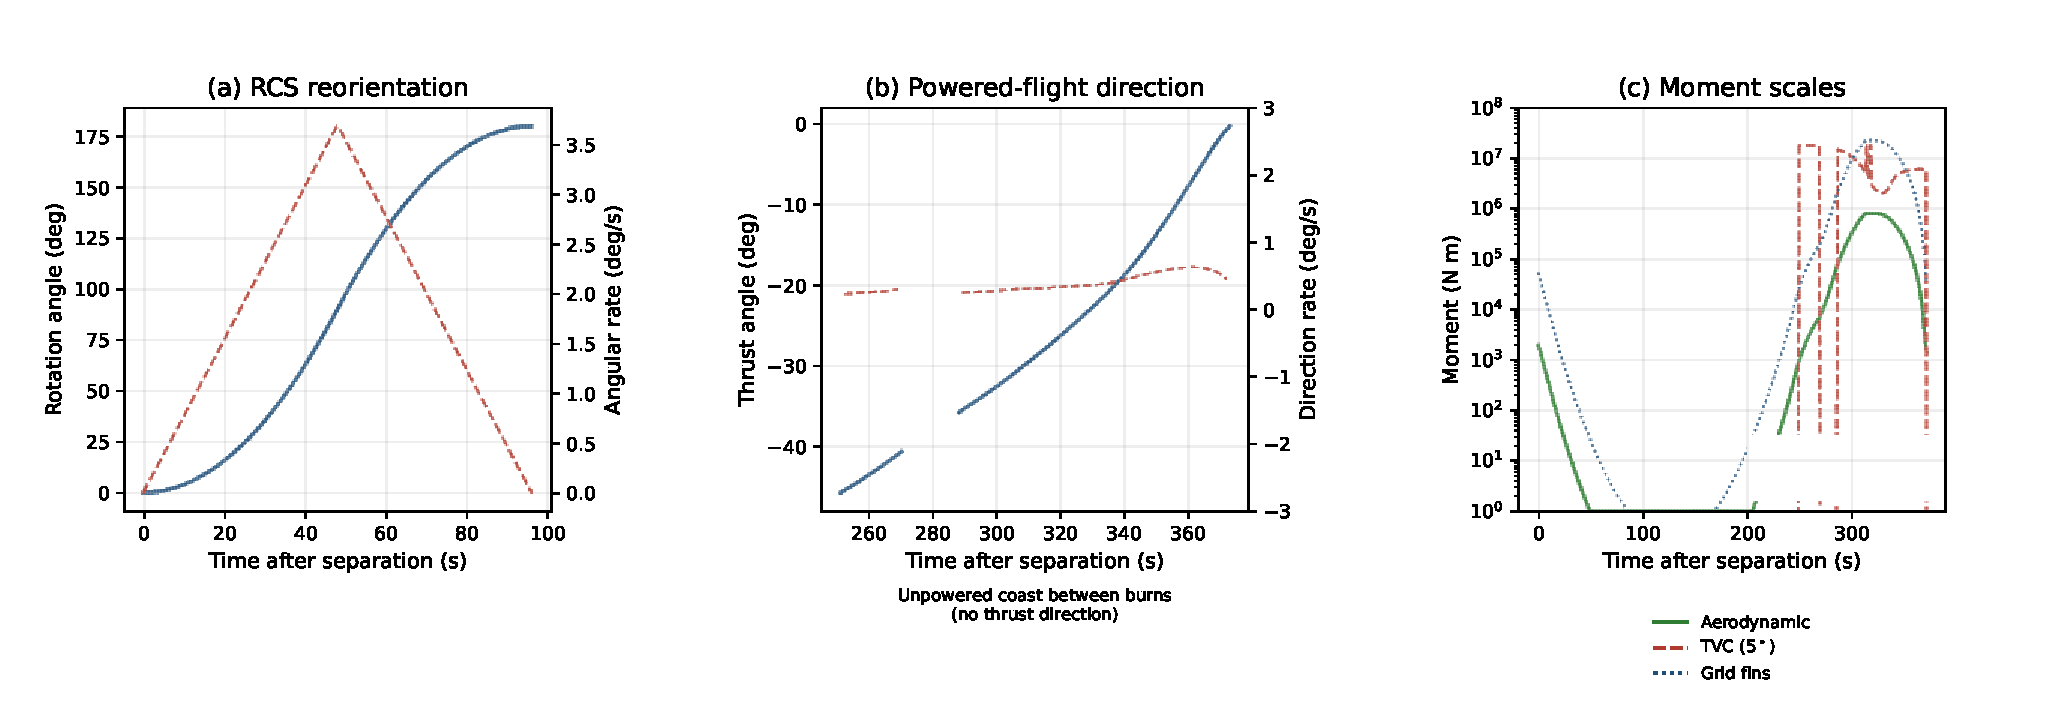
\includegraphics[width=\linewidth]{attitude_relayout.pdf}
\caption{Attitude and moment-scale estimates. (a) One-degree-of-freedom RCS reorientation. (b) Required thrust direction during powered flight; the gap corresponds to the unpowered coast. (c) Aerodynamic, TVC, and estimated grid-fin moment scales. The traces are reproduced from plot pixels without reconstructing obscured portions. These separate estimates do not constitute a fully coupled attitude solution.}
\label{fig:attitude}
\end{figure}

The analysis additionally gives a grid-fin moment estimate of 22.8 MN m and compares its reported direction-slew requirement of 0.63$^\circ$/s with a 5$^\circ$/s reference limit.

The ratio of the reported 18.3 MN m TVC scale to the 0.83 MN m aerodynamic scale is about 22. Such a magnitude comparison can motivate further modeling, but does not by itself establish simultaneous force and torque feasibility, bandwidth, rate limits, or closed-loop stability. The direction-slew estimate and the separate RCS maneuver do not resolve a fully coupled rotational history.

\subsection{Jet-interaction parameterization}
The model uses a thrust-coefficient-based correction,
\begin{equation}
 C_T=\frac{T}{qA},\qquad
 C_D^{eff}=C_D(M)\left[1+k_{jet}\frac{C_T}{1+C_T}\right].
\label{eq:jet}
\end{equation}
The tested $k_{jet}$ values are 0, 0.3, and 0.6. Retropropulsion and grid-fin literature provide the physical context for considering such effects \cite{retro,korzun,gridfin}, but the chosen coefficients are scenario parameters rather than a calibrated database for this booster.

\begin{table}[htbp]
\caption{Simulation jet-interaction sensitivity at 120 t initial load.}
\label{tab:src12}
\small
\setlength{\tabcolsep}{3.5pt}
\begin{tabularx}{\linewidth}{@{}rrrr@{}}
\toprule
Jet coefficient & Entry (t) & Landing (t) & Total (t) \\
\midrule
0 & 42.4 & 70.5 & 112.9 \\
0.3 & 42.4 & 69.5 & 111.9 \\
0.6 & 42.4 & 69.6 & 112.0 \\
\bottomrule
\end{tabularx}
\par\smallskip{\footnotesize Totals are calculated from the displayed phase consumptions. The jet coefficient is a parametric assumption, not a CFD-calibrated property of the booster.}
\par\smallskip{\footnotesize Belongs to v1-J. See \cref{tab:versions}.}
\end{table}

\begin{table}[htbp]
\caption{Summary of separate model extensions.}
\label{tab:src13}
\small
\setlength{\tabcolsep}{3.5pt}
\begin{tabularx}{\linewidth}{@{}XXXX@{}}
\toprule
Model & Propellant at 120 t & Touchdown & Qualification \\
\midrule
2D reference & 113.0 t & 2.5 m/s & Ideal attitude, no jet correction \\
3D with crosswind & 111.9 t & 2.5 m/s & 0.35 km cross-track drift \\
3D jet-parameter cases & 111.9--112.9 t & 2.5 m/s & About 1 t variation \\
Simulation load recommendation & 112 t & 2.5 m/s & 120 t includes tested disturbance allowance \\
\bottomrule
\end{tabularx}
\par\smallskip{\footnotesize The 113.0 t two-dimensional reference (v1-D2) and 111.8 t pre-search comparator (v1-P) are distinct calculation series and are not interchangeable; the crosswind and jet cases are v1-D3 and v1-J. See \cref{tab:versions}.}
\end{table}


The calculations indicate approximately 1 t variation across the listed jet cases. The analysis does not calculate bottom heating, surface pressure distribution, or reusable thermal protection. The limited fuel difference does not quantify the magnitude of thermal or structural effects.

\section{Parameterized Guidance Optimization}
\subsection{Search method and decision variables}
The four-parameter direct shooting search uses SciPy's derivative-free Powell method and grid refinement. CasADi/IPOPT is not used for these results.

\begin{table}[htbp]
\caption{Four variables in the reported Powell and grid search.}
\label{tab:src14}
\small
\setlength{\tabcolsep}{3.5pt}
\begin{tabularx}{\linewidth}{@{}lXr@{}}
\toprule
Variable & Meaning & Range \\
\midrule
$h_e$ & Entry-ignition height & 35--82 km \\
$v_{cut}$ & Entry cutoff speed & 450--1150 m/s \\
$k$ & Landing-ignition height multiplier & 0.95--1.60 \\
$V_{td}$ & Target touchdown speed & 0.5--3.0 m/s \\
\bottomrule
\end{tabularx}
\par\smallskip{\footnotesize Search domain for v3-P. See \cref{tab:versions}.}
\end{table}


The parameters are entry ignition height $h_e$, entry cutoff speed $v_{cut}$, the terminal-ignition multiplier $k$, and target speed $V_{td}$. Each trial corresponds to a simulated trajectory with those rules. The model describes the penalty objective as
\begin{equation}
 J=\dot m\,t_{burn}
 +50\max(0,V_{touch}-2.5)
 +2\max(0,q_{max}-50\ \mathrm{kPa}).
\label{eq:objective}
\end{equation}
The weights are empirical numerical penalties. Feasibility is evaluated separately using the dimensional touchdown-speed, dynamic-pressure, and propellant limits, rather than inferred from the penalty value alone. This is a parameterized guidance search with penalties, not a demonstrated solution of the unrestricted continuous optimal-control problem.

The reported constraints are touchdown speed below 2.5 m/s, peak dynamic pressure at most 50 kPa, and no consumption beyond the carried load. A run that exhausts propellant before meeting the terminal requirement is counted as a failure.

\subsection{Late and shorter entry pulse}
\begin{table}[htbp]
\caption{Simulation comparison between baseline and parameterized guidance.}
\label{tab:src15}
\small
\setlength{\tabcolsep}{3.5pt}
\begin{tabularx}{\linewidth}{@{}p{.34\linewidth}XX@{}}
\toprule
Item & Baseline comparator (v1-P) & Parameterized search (v3-P) \\
\midrule
Entry burn & 75 to 55 km; about 42 t & 55 to 40 km; about 27 t \\
Terminal braking & From about 47 km; 70--121 t & Pressure-triggered; 69--87 t \\
Lowest reported feasible load & 104 t (v1-B scan) & 96 t (v3-P) \\
Consumption at 120 t & 111.8 t & 108.5 t \\
Peak pressure & 47.6 kPa & 47.6 kPa \\
\bottomrule
\end{tabularx}
\par\smallskip{\footnotesize The comparison columns are v1-P and v3-P. The 104 t threshold refers to the separate v1-B fine scan; it does not identify the 120 t comparator as an identical simulation. See \cref{tab:versions}.}
\end{table}


The v3-P parameterized solution (\cref{tab:versions}) moves entry ignition downward from 75 km to about 55 km and ends the pulse near 40 km. Entry propellant decreases from roughly 42 t to 27 t in that comparison. The analysis attributes the saving to avoiding an extended high-altitude burn where aerodynamic braking is weak and gravity continues to act during thrusting.

This explanation is specific to the guidance strategy and its constraints. Delaying ignition too far can also remove the remaining stopping distance or increase the pressure peak. Reusable-launcher guidance literature motivates the interaction of timing, control, and terminal requirements \cite{wilken,simplicio,botelho}; it does not turn the finite parameter search into a global optimum proof.

\subsection{Reported optimized disturbance allowance}
\begin{table}[htbp]
\caption{Simulation perturbation results for parameterized guidance. Numeric successful entries are consumed propellant in tonnes.}
\label{tab:src16}
\small
\setlength{\tabcolsep}{3.5pt}
\begin{tabularx}{\linewidth}{@{}rXXXXX@{}}
\toprule
Load (t) & Nominal & $C_D-15\%$ & $C_D-20\%$ & $I_{sp}-2\%$ & Combined \\
\midrule
96 t & Pass: 95.9 & Fail & Fail & Fail & Fail \\
104 t & Pass: 100.2 & Fail & Fail & Pass & Fail \\
110 t & Pass: 103.3 & Pass: 107.3 & Pass: 108.7 & Pass: 104.6 & Pass: 108.8 \\
112 t & Pass: 104.4 & Pass: 108.3 & Pass: 109.7 & Pass: 105.7 & Pass: 109.8 \\
\bottomrule
\end{tabularx}
\par\smallskip{\footnotesize Belongs to v3-P. See \cref{tab:versions}.}
\end{table}


Under v3-P parameterized guidance (\cref{tab:versions}), the study reports 96 t as the lowest nominal successful load in its test, while 110 t passes the selected optimized perturbations. At 110 t, reported consumed propellant is 103.3 t nominally and 108.8 t in the combined case. At 112 t these numbers are 104.4 t and 109.8 t. The numerical entries represent consumed propellant, whereas parenthesized successful values in the baseline perturbation table represent residual mass; they describe different mass quantities.

\begin{figure}[htbp]
\centering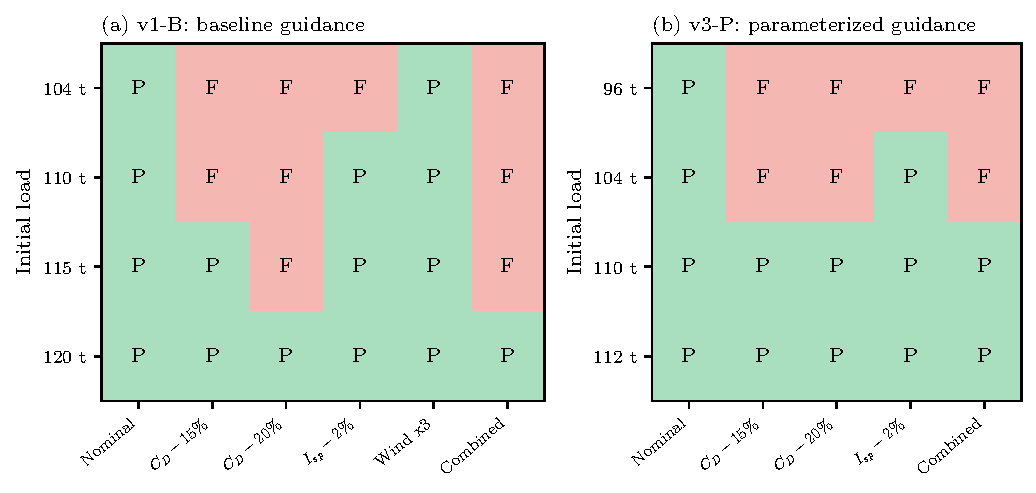
\includegraphics[width=\linewidth]{source_perturbation_matrix.pdf}
\caption{Pass/fail patterns for the tested cases: (a) baseline guidance and (b) parameterized guidance. P and F denote the model's reported outcomes. These are categorical views of the tabulated results, not new simulation runs or probability estimates.}
\label{fig:matrix}
\end{figure}

\section{Area Coupling, Engine Response, and Staging}
\label{sec:refinements}
\subsection{Attitude-dependent effective area}
The final model refinement replaces a fixed reference area with
\begin{equation}
 A_{eff}=A\cos^2\alpha+(Ld)\sin^2\alpha,
 \qquad A=38.48\ \mathrm{m}^2,\quad Ld=455\ \mathrm{m}^2.
\label{eq:area}
\end{equation}
A first-order attitude lag with a reference time constant of 1 s allows a mismatch between the prescribed alignment and body direction. Without any mismatch, an ideal alignment model could hide the influence of the area law. A separate comparison tests a 3 s lag in its later comparison.

\begin{table}[htbp]
\caption{Simulation area-law comparison before the final combined model.}
\label{tab:src17}
\small
\setlength{\tabcolsep}{3.5pt}
\begin{tabularx}{\linewidth}{@{}rXXXX@{}}
\toprule
Load (t) & Without area law (t) & With area law (t) & Difference (t) & $q_{\max}$ (kPa) \\
\midrule
110 & 109.2 & 107.8 & -1.4 & 45.6 \\
120 & 114.8 & 113.5 & -1.3 & 44.7 \\
\bottomrule
\end{tabularx}
\par\smallskip{\footnotesize Belongs to the v3-I reference and its area-only variant v3-A. See \cref{tab:versions}.}
\end{table}


The results indicate fuel reductions of about 1.3--1.4 t in these particular area-law cases. Increased projected area can provide additional drag, but this is not a general claim that attitude error is beneficial: loads, torques, heating, and control feasibility can also change. The analysis does not provide a complete validated aerodynamic force-and-moment model for those effects.

\subsection{Design and acceptance pressure thresholds}
The later model uses a 47 kPa guidance trigger and a 50 kPa acceptance screen. Its listed pressure peaks lie around 44.7--45.6 kPa, leaving roughly 5 kPa below the acceptance value. This is an assigned design gap, not a quantified confidence interval for drag and wind uncertainty.

\subsection{Finite response and the throttle-floor problem}
The refined model adds a 0.5 s ignition delay, a 0.1 s first-order response, and a throttle slew limit of $1$ s$^{-1}$. In its first attempt at this refinement, 110 t and 120 t cases exhausted propellant and reached reported terminal speeds of roughly 160--180 m/s.

The subsequent diagnosis identifies the throttle floor rather than delay alone as a central difficulty. The terminal law requested only about 10--18\% of the seven-engine nominal thrust, while seven simultaneously enabled engines at 30\% supply 2.1 MN. The model describes excessive braking, a low-speed condition near 2.6 km, renewed descent, and eventual exhaustion.

The reported remedy is staged engine selection: seven engines during entry, three in the intermediate part, and one in the late terminal portion. Each enabled engine retains the stated 30--110\% throttle range. This reduces absolute thrust increments and permits finer terminal modulation. It is a change in the control arrangement, not evidence that a single engine can hover against the dry weight; a short transient arrival and a stable supported landing are different questions.

\subsection{Combined results and final propellant recommendation}
\begin{table}[htbp]
\caption{Simulation ablation of area law, finite engine response, and engine-count staging.}
\label{tab:src18}
\small
\setlength{\tabcolsep}{3.5pt}
\begin{tabularx}{\linewidth}{@{}p{.36\linewidth}XXXX@{}}
\toprule
Model & Fuel at 110 t & Fuel at 120 t & $V_{td}$ (m/s) & $q_{\max}$ (kPa) \\
\midrule
Ideal v3 reference & 109.2 t & 114.8 t & 2.40 & 45.6 \\
Area law added & 107.8 t & 113.5 t & 2.46 & 45.6 \\
Engine response and staging & 109.0 t & 114.7 t & 1.96 & 44.9 \\
Both effects: final v4-F & 106.6 t & 112.7 t & 2.02 & 44.9 \\
Combined, attitude lag $\tau=3$ s & 107.9 t & 113.7 t & 2.01 & 44.7 \\
\bottomrule
\end{tabularx}
\par\smallskip{\footnotesize Rows are v3-I, v3-A, v4-R, v4-F, and v4-L, respectively; these ablation cases differ from v3-P. See \cref{tab:versions}.}
\end{table}


\begin{figure}[htbp]
\centering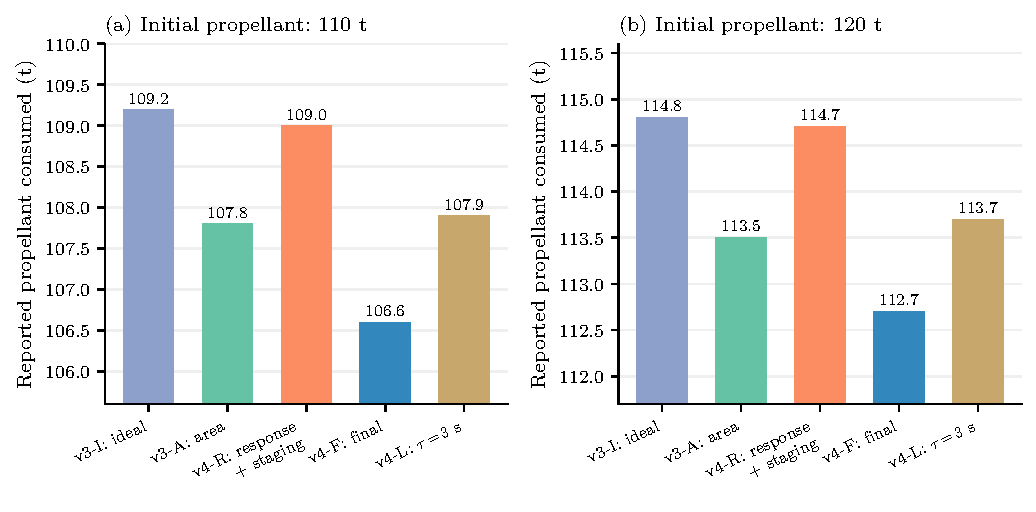
\includegraphics[width=\linewidth]{source_ablation.pdf}
\caption{Fuel consumption for the labeled ablation variants (v3-I through v4-L in \cref{tab:versions}) at (a) 110 t and (b) 120 t initial propellant. Values are plotted directly from the ablation table. Adding engine response also changes engine-count staging, so the difference is not an isolated physical effect of response delay alone.}
\label{fig:ablation}
\end{figure}

In the final v4-F series (\cref{tab:versions}), at 110 t initial propellant the combined model consumes 106.6 t, leaving 3.4 t of residual propellant.

The final combined v4-F row reports 106.6 t consumption at 110 t initial load and 112.7 t at 120 t, with a 2.02 m/s touchdown entry and 44.9 kPa pressure peak in the summary. The separate 3 s attitude-lag variant consumes more than the 1 s reference. Each comparison refers to one specified model version and its corresponding control settings.

\begin{table}[htbp]
\caption{Simulation final load scan with area law, finite response, and staged engine selection.}
\label{tab:src19}
\small
\setlength{\tabcolsep}{3.5pt}
\begin{tabularx}{\linewidth}{@{}rrrr@{}}
\toprule
Load (t) & Outcome & Consumed (t) & $V_{td}$ (m/s) \\
\midrule
96 t & Fail & 96.0 & 37.5 m/s \\
100 t & Fail & 100.0 & 11.3 m/s \\
102 t & Pass & 101.7 & 2.02 m/s \\
110 t & Pass & 106.6 & 2.02 m/s \\
120 t & Pass & 112.7 & 2.00 m/s \\
\bottomrule
\end{tabularx}
\par\smallskip{\footnotesize Belongs to final series v4-F. See \cref{tab:versions}.}
\end{table}


The final v4-F load scan in \cref{tab:src19,tab:versions} records 96 t and 100 t as unsuccessful, followed by 102 t arriving at 2.02 m/s after consuming 101.7 t. Its recommendation is 110--112 t, retaining an allowance above the lowest reported passing case. The earlier 96 t value belongs to the more idealized parameterized model, while the earlier 104 t value belongs to baseline guidance.


\FloatBarrier
\begin{table}[!htbp]
\centering
\caption{Register of calculation series and consumed propellant. The final recommendation belongs to v4-F.}
\label{tab:versions}
\small
\setlength{\tabcolsep}{4pt}
\begin{tabularx}{\linewidth}{@{}lXrr@{}}
\toprule
Series & Calculation and role & At 110 t & At 120 t\\
\midrule
v1-B & Baseline load scan, 75 km entry ignition & 107.2 t & ---\\
v1-D2 & 2D reference for the crosswind diagnostic & --- & 113.0 t\\
v1-D3 & 3D crosswind diagnostic & --- & 111.9 t\\
v1-J & Jet-interaction sensitivity cases & --- & 111.9--112.9 t\\
v1-P & Pre-search comparator in the guidance comparison & --- & 111.8 t\\
v3-P & Parameterized guidance, entry ignition near 55 km & 103.3 t & 108.5 t\\
v3-I & Ideal reference in the actuator/area ablation & 109.2 t & 114.8 t\\
\textbf{v4-F} & \textbf{Combined final model; recommended design} & \textbf{106.6 t} & \textbf{112.7 t}\\
\bottomrule
\end{tabularx}
\par\smallskip{\footnotesize Column headings indicate initial total propellant, while entries indicate consumption. A dash denotes no value tabulated for that series. The v1-B entry at 110 t is the displayed phase sum $42.7+64.5=107.2$ t; v1-D3 and v1-J also use displayed phase sums. Suffixes identify separate calculation series, not inferred equivalence of controllers or atmosphere settings. v3-A, v4-R, and v4-L denote the area-only, response/staging-only, and 3 s lag variants within the ablation comparison.}
\end{table}

\noindent\Cref{tab:versions} separates nominal load, consumed propellant, and calculation series. In particular, the 113.0 t two-dimensional diagnostic comparator (v1-D2) and the 111.8 t pre-search comparator (v1-P) are distinct records with no demonstrated identical configuration; neither is substituted for the other. The 111.9 t crosswind value is v1-D3, and the final 112.7 t consumption at 120 t load belongs to v4-F. The ideal ablation reference v3-I also differs from the parameterized guidance series v3-P, despite both being associated with the third modeling stage. The final recommendation refers only to v4-F: 110--112 t initial propellant, with 106.6 t consumed and 2.02 m/s touchdown at the 110 t case. The separate 120 t case consumes 112.7 t and reaches 2.00 m/s in the final load scan.

\begin{figure}[htbp]
\centering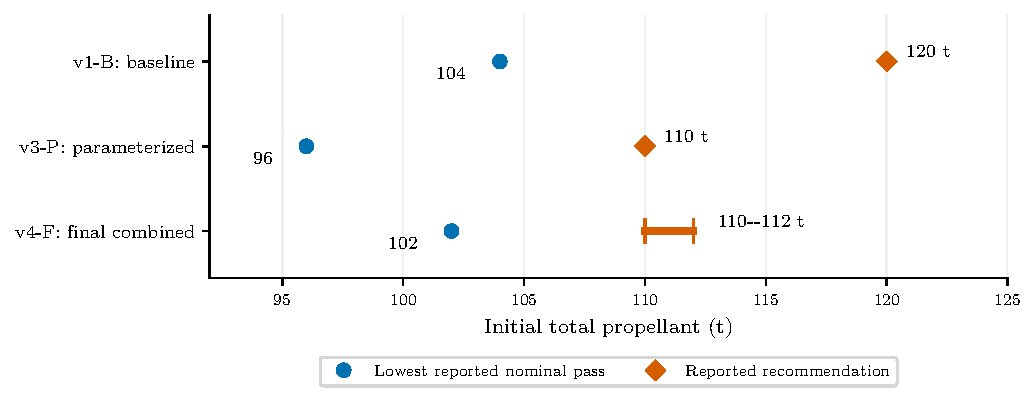
\includegraphics[width=\linewidth]{source_load_summary.pdf}
\caption{Version-specific load thresholds and recommendations reported in the study. The circles are the lowest reported nominal passes; the recommendations refer to their respective reported test sets or design allowances. Different model and acceptance settings prevent interpreting this as a universal ranking of minimum fuel.}
\label{fig:loads}
\end{figure}

\section{Discussion: Strengths and Limitations}
\subsection{Physical interpretation of the study trends}
Three recurring effects organize the results. First, entry and terminal burns play different roles: the baseline entry pulse removes a modest part of the speed, while terminal braking must close the remaining velocity and altitude budget. Second, additional propellant changes the mass being decelerated, so a heavier initial load can require earlier braking and consume much of the added mass. Third, state-dependent guidance must be compatible with absolute thrust floors, finite response, and the number of active engines.

The model's wind comparison also separates fuel efficiency from landing accuracy. Similar consumed mass does not imply similar lateral speed or range. Its area and jet investigations show why a change in aerodynamic representation can alter the apparent fuel requirement even without changing the basic dimensions or propellant species.

\subsection{Strengths of the modeling sequence}
The study compares several physically motivated refinements instead of presenting one unexplained fuel number. It distinguishes air-relative and ground-relative velocities, shows representative stage histories, includes finite perturbation sets, and diagnoses a throttle-floor problem that an ideal continuous-thrust law can hide. Keeping separate tables for baseline guidance, parameterized guidance, and actuator refinements makes those comparisons interpretable.

The separate RCS and moment estimates provide useful scale checks, while the three-dimensional example highlights cross-track motion absent from the simplest plane model. These are useful components of further analysis, even though they do not collectively demonstrate a complete closed-loop recovery simulation.

\subsection{Limitations and evidence still required}
The numerical results have not been independently rerun. Complete executable programs, $C_D(M)$ anchor values, high-altitude extension details, and penalty normalization are required for independent numerical reproduction.

The displayed velocity equations and angular definitions require implementation review, as described in \cref{eq:sourceforces,eq:sourcetrigger}. Peak load factor is reported in the load scan, but a full stress distribution, structural capacity, and thermal-protection analysis are not available. No temperature history is manufactured from the pressure result.

The early ideal-engine and ideal-alignment assumptions do not apply to every late model. Conversely, the later throttle range, delay, and lag do not establish engine-out behavior or actual flight hardware capability. The model's one-dimensional attitude estimates are post hoc, and the final first-order lag is not a complete coupled rigid-body controller. Deployment, actual foot velocities, deck motion, leg compression, friction, and post-contact stability remain outside the demonstrated result.

Finally, finite successful perturbation sets justify only their tested cases. They do not establish a failure probability, a confidence interval, or a universal robustness margin. The combined refined model's 110--112 t recommendation is conditional on the modeled guidance and tested perturbations; it is not a quantified probabilistic safety bound.

\section{Conclusion}
This simulation study describes the return of a seven-engine, 130 t dry-mass booster from 70 km and 6,000 km/h with an initial upward flight-path angle of $45^\circ$. Its reported ascent reaches about 143 km before the entry and terminal burns complete the descent. Baseline entry propellant remains near 40--44 t, while terminal consumption grows strongly with carried mass.

The development-stage comparisons are organized in \cref{tab:versions}; the final recommendation is the v4-F separation load of 110--112 t. The intermediate thresholds depend on calculation series. Baseline guidance reports a lowest passing tested load of 104 t and a disturbance-tested recommendation of 120 t. Parameterized Powell/grid guidance reports 96 t nominally and recommends 110 t for its chosen tests. The later combined area-law, finite-response, and staged-engine model reports a 102 t nominal passing case and recommends 110--112 t. At 110 t its summary gives 106.6 t consumed and 2.02 m/s touchdown speed.

The results highlight the interaction of ignition timing, mass, drag, throttle floor, and engine selection. They remain empirical results of the tested models rather than mathematical global minima or a demonstration of complete shipboard landing safety.

\clearpage
\section{AI Usage Report}
\label{sec:ai}
\subsection{System Used}
OpenAI ChatGPT with Codex tools was used as an assistant during the preparation of this paper. The exact deployed model version is not recorded in the available conversation archive.

\subsection{Scope and Nature of Use}
The system assisted with discussion of physical assumptions and numerical methods, equation and unit checks, identification of references, translation and academic editing, and LaTeX preparation. It also helped arrange figures and tables, insert the uploaded recovery photograph, and prepare the explanatory Python listings in Appendix~\ref{app:code}. The photograph was extracted from the supplied image archive and was not generated or retouched by the AI system.

\subsection{Content Authorship}
The trajectory tables and numerical conclusions correspond to the calculation series identified in \cref{tab:versions}. AI assistance also contributed to the method explanations and reference-code implementation; it was not confined to grammar correction. The new listings are explanatory components rather than the programs that generated the flight tables. Their tests therefore do not establish independent reproduction of the mission results. Responsibility for the scientific content, interpretation, and final submission remains with Team~\TeamNumber.

\subsection{Quality Assurance}
The final LaTeX document was compiled and checked for unresolved references, missing characters, layout overflow, consistent team numbering, and the five-page code appendix. The reference code was checked against smooth-ODE RK4 convergence, thrust--mass-flow consistency, drag direction, fuel-exhaustion handling, touchdown interpolation, and a bounded search test. These checks have a narrower scope than full trajectory validation. Retained exchanges are archived in the accompanying electronic materials.


\clearpage
\phantomsection
\addcontentsline{toc}{section}{References}
\begin{thebibliography}{14}
\small
\bibitem{problem} University Physics Competition. \emph{2026 Problems}, Problem A.
\bibitem{ussa} NOAA/NASA/USAF. \emph{U.S. Standard Atmosphere, 1976}. NASA-TM-X-74335, 1976.
\bibitem{earth} NASA NSSDC. \emph{Earth Fact Sheet}.
\bibitem{iers} IERS. \emph{IERS Conventions (2010)}, TN 36.
\bibitem{retro} A. Marwege et al. Hypersonic retro propulsion for reusable launch vehicles tested in the H2K wind tunnel. \emph{CEAS Space Journal}, 14:473--499, 2022. DOI: \url{https://doi.org/10.1007/s12567-022-00457-w}.
\bibitem{korzun} A. M. Korzun and R. D. Braun. Conceptual modeling of supersonic retropropulsion flow interactions. \emph{Journal of Spacecraft and Rockets}, 50:1121--1133, 2013. DOI: \url{https://doi.org/10.2514/1.A32464}.
\bibitem{wilken} J. Wilken and S. Stappert. Comparative analysis of European vertical landing reusable first stage concepts. \emph{CEAS Space Journal}, 17:113--130, 2025. DOI: \url{https://doi.org/10.1007/s12567-024-00549-9}.
\bibitem{simplicio} P. Simpl\'{i}cio, A. Marcos, and S. Bennani. Guidance of reusable launchers: improving descent and landing performance. \emph{Journal of Guidance, Control, and Dynamics}, 42:2206--2219, 2019. DOI: \url{https://doi.org/10.2514/1.G004155}.
\bibitem{botelho} A. Botelho et al. Design of the landing guidance for the retro-propulsive vertical landing of a reusable rocket stage. \emph{CEAS Space Journal}, 14:551--564, 2022. DOI: \url{https://doi.org/10.1007/s12567-022-00423-6}.
\bibitem{gridfin} P. Theerthamalai and M. Nagarathinam. Aerodynamic analysis of grid-fin configurations at supersonic speeds. \emph{Journal of Spacecraft and Rockets}, 43:750--756, 2006. DOI: \url{https://doi.org/10.2514/1.16741}.

\bibitem{hairer} E. Hairer, S. P. N\o rsett, and G. Wanner. \emph{Solving Ordinary Differential Equations I: Nonstiff Problems}. 2nd ed., Springer, 1993. DOI: \url{https://doi.org/10.1007/978-3-540-78862-1}.
\bibitem{powell} M. J. D. Powell. An efficient method for finding the minimum of a function of several variables without calculating derivatives. \emph{The Computer Journal}, 7(2):155--162, 1964. DOI: \url{https://doi.org/10.1093/comjnl/7.2.155}.
\bibitem{scipy} SciPy Developers. \emph{minimize(method='Powell')}. \url{https://docs.scipy.org/doc/scipy/reference/optimize.minimize-powell.html}.
\bibitem{airules} University Physics Competition. \emph{Contest Rules}, Solution Papers and Generative AI. Accessed 8 November 2026. \url{https://www.uphysicsc.com/contestrules.html}.

\end{thebibliography}


\clearpage
\appendix
\section{Reference Code Listings}
\label{app:code}
\noindent The following five pages present reference components, not a reproduction of the tabulated flight results. Environmental tables are external inputs. Basic identity tests accompany the electronic package; full trajectory validation remains separate.
\lstset{language=Python,basicstyle=\ttfamily\fontsize{9}{10.5}\selectfont,numbers=left,numberstyle=\tiny,numbersep=6pt,frame=single,breaklines=true,columns=fullflexible,keepspaces=true,showstringspaces=false,tabsize=4,xleftmargin=12pt,xrightmargin=3pt,aboveskip=5pt,belowskip=4pt}
\subsection*{Listing A.1. Constants and environmental interfaces}
\lstinputlisting{code/environment.py}
\clearpage
\subsection*{Listing A.2. Aerodynamic force and translational equations}
\lstinputlisting{code/dynamics.py}
\clearpage
\subsection*{Listing A.3. RK4 and touchdown interpolation}
\lstinputlisting{code/integrator.py}
\noindent\small The command is held over each substep. Thus fourth-order accuracy of RK4 on a smooth prescribed right-hand side does not imply fourth-order accuracy of the entire switched, sampled-control trajectory.
\clearpage
\subsection*{Listing A.4. Illustrative two-burn guidance}
\lstinputlisting{code/guidance.py}
\noindent\small This explanatory policy omits the later actuator lag and engine-count staging and uses a stopping-distance trigger. It is not the final combined-model simulator.
\clearpage
\subsection*{Listing A.5. Bounded Powell search and local grid}
\lstinputlisting{code/search.py}
\noindent\small The evaluator returns terminal metrics. The normalized penalty is illustrative; strict physical feasibility is evaluated separately from the penalty value.
\normalsize
\end{document}
